%%%%%%%%%%%%%%%%%%%%%%%%%%%%%%%%%%%%%%%%%
% Jacobs Landscape Poster
% LaTeX Template
% Version 1.1 (14/06/14)
%
% Created by:
% Computational Physics and Biophysics Group, Jacobs University
% https://teamwork.jacobs-university.de:8443/confluence/display/CoPandBiG/LaTeX+Poster
% 
% Further modified by:
% Nathaniel Johnston (nathaniel@njohnston.ca)
%
% This template has been downloaded from:
% http://www.LaTeXTemplates.com
%
% License:
% CC BY-NC-SA 3.0 (http://creativecommons.org/licenses/by-nc-sa/3.0/)
%
%%%%%%%%%%%%%%%%%%%%%%%%%%%%%%%%%%%%%%%%%

%----------------------------------------------------------------------------------------
%	PACKAGES AND OTHER DOCUMENT CONFIGURATIONS
%----------------------------------------------------------------------------------------

\documentclass[10pt]{beamer}
%\usepackage[utf8]{inputenc}
\usepackage[small]{optional}% use small or large

\usepackage[scale=1.4]{beamerposter} % Use the beamerposter package for laying out the poster
\usepackage{palatino} 
\usepackage{textpos}
\usetheme{confposter} % Use the confposter theme supplied with this template

\setbeamercolor{block title}{fg=ngreen,bg=white} % Colors of the block titles
\setbeamercolor{block body}{fg=black,bg=white} % Colors of the body of blocks
\setbeamercolor{block alerted title}{fg=white,bg=dblue!70} % Colors of the highlighted block titles
\setbeamercolor{block alerted body}{fg=black,bg=dblue!20} % Colors of the body of highlighted blocks
\setbeamercolor{background canvas}{fg=black,bg=dblue!10} 
% Many more colors are available for use in beamerthemeconfposter.sty

%-----------------------------------------------------------
% Define the column widths and overall poster size
% To set effective sepwid, onecolwid and twocolwid values, first choose how many columns you want and how much separation you want between columns
% In this template, the separation width chosen is 0.024 of the paper width and a 4-column layout
% onecolwid should therefore be (1-(# of columns+1)*sepwid)/# of columns e.g. (1-(4+1)*0.024)/4 = 0.22
% Set twocolwid to be (2*onecolwid)+sepwid = 0.464
% Set threecolwid to be (3*onecolwid)+2*sepwid = 0.708

\newlength{\sepwid}
\newlength{\onecolwid}
\newlength{\twocolwid}
\newlength{\threecolwid}
\setlength{\paperwidth}{48in} % A0 width: 46.8in
\setlength{\paperheight}{36in} % A0 height: 33.1in
\setlength{\sepwid}{0.024\paperwidth} % Separation width (white space) between columns
\setlength{\onecolwid}{0.22\paperwidth} % Width of one column
\setlength{\twocolwid}{0.464\paperwidth} % Width of two columns
\setlength{\threecolwid}{0.708\paperwidth} % Width of three columns
\setlength{\topmargin}{-0.5in} % Reduce the top margin size
%-----------------------------------------------------------http://dmi.unibas.ch/

\usepackage{graphicx}  % Required for including images

%----------------------------------------------------------------------------------------
%	TITLE SECTION 
%----------------------------------------------------------------------------------------

\title{\LARGE Why is it so hard to send unobservable messages across the internet?} % Poster title

\author{Martin Gwerder (m.gwerder@unibas.ch)} % Author(s)

\institute{Department of Mathematics and Computer Science, University of Basel} % Institution(s)
 
%----------------------------------------------------------------------------------------

%{\usebackgroundtemplate{%
%
\includegraphics[width=1.2\paperwidth,height=1.7\paperheight]{bg_image}%
%}
\addtobeamertemplate{block end}{}{\vspace*{2ex}} % White space under blocks
\addtobeamertemplate{block alerted end}{}{\vspace*{2ex}} % White space under highlighted (alert) blocks

\setlength{\belowcaptionskip}{2ex} % White space under figures
\setlength\belowdisplayshortskip{2ex} % White space under equations

\begin{document}%
\begin{frame}[t] % The whole poster is enclosed in one beamer frame

\begin{columns}[t] % The whole poster consists of three major columns, the second of which is split into two columns twice - the [t] option aligns each column's content to the top

\begin{column}{\sepwid}\end{column} % Empty spacer column

\begin{column}{\onecolwid} % The first column

%----------------------------------------------------------------------------------------
%	OBJECTIVES
%----------------------------------------------------------------------------------------

\begin{alertblock}{Objectives}

This work emphasizes on the requirements needed to create a system that is capable to transfer unobserved messages across the internet. It focusses on:
\begin{itemize}
\item What is required to create unobservable messages?
\item What parts are already available as well established technologies?
\item Where do we have a lack of reliable and researched technologies?
\end{itemize}

In this poster, I emphasize on the result. If you are interested at the argumentation, I recommend the corresponding paper referenced at the lower right for further reading.

\end{alertblock}

%----------------------------------------------------------------------------------------
%	INTRODUCTION
%----------------------------------------------------------------------------------------
\vfill
\begin{block}{Introduction}

There are lots of works\cite{tor-design}\cite{mixmaster-spec}\cite{xor-trees}\cite{Levine:2002} that relate to anonymous message transfer. However -- none of these works (with exception to TOR\cite{tor-design}) has been widely adopted in the internet. The reason for this is usually that peoples tend to concentrate on the method to transport the message and fail at the same time completely to take the real world and its problems into account. I collected some information that helps to create sensible and reliable systems. 

\begin{figure}
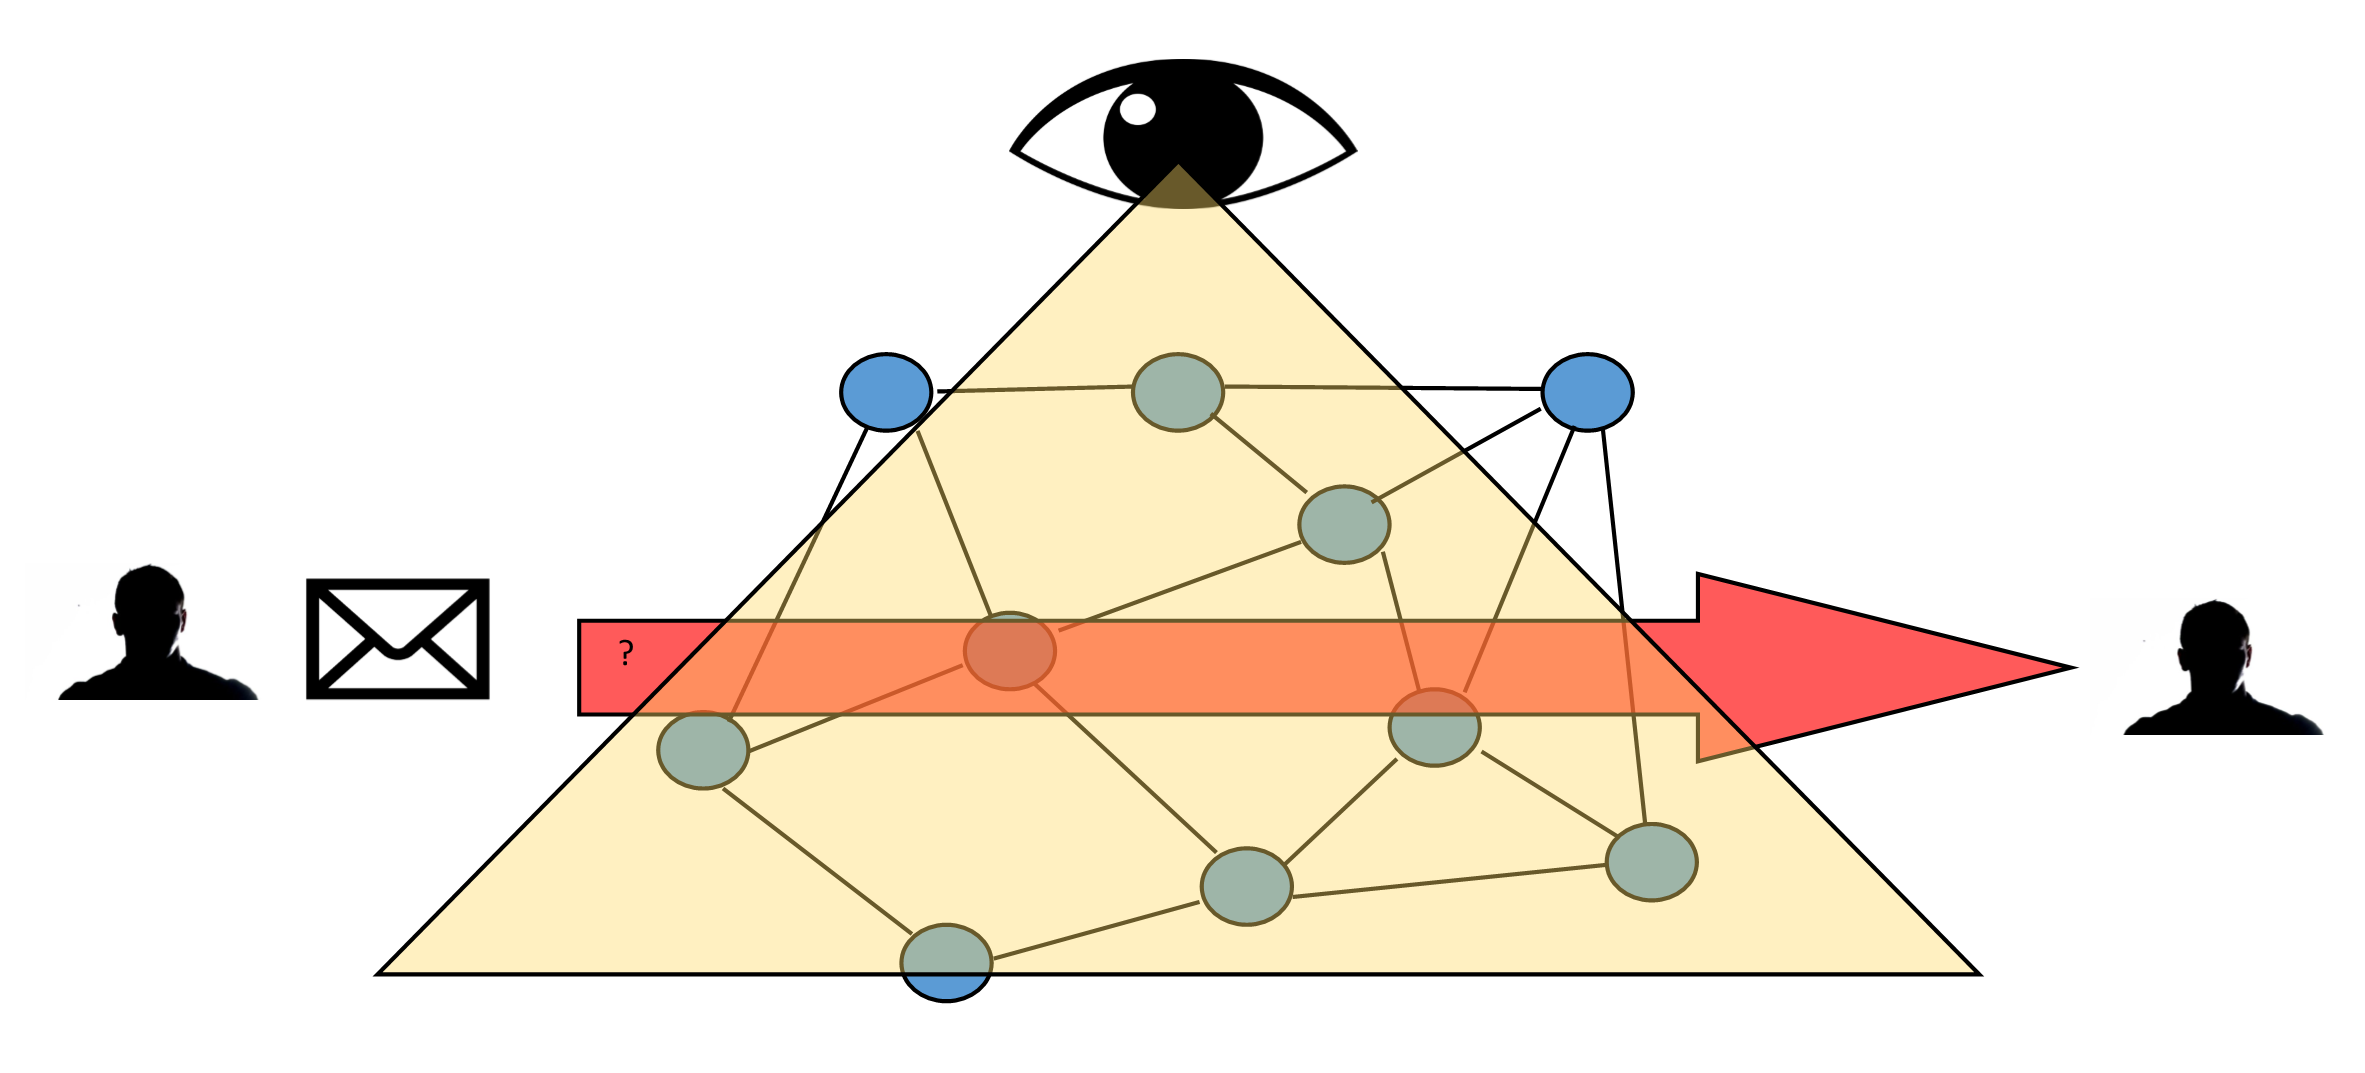
\includegraphics[width=0.9\linewidth]{messagetransfer.png}
\caption{sending unobservable messages is not easy}
\end{figure}
\end{block}

\vfill
\begin{block}{Categorisation}

In order to simplify the aspects of unobservability I categorized them into three categories. 

\begin{itemize}
\item Acceptance \opt{large}{\\
      What properties are expected from a user perspective? A ``user'' might be any participant (eg sender, recipient, or infrastructure administrator) except the suspected observer.}
\item Protocol\opt{large}{\\
      What properties are expected when looking at the communication protocol? This point spans across all layers of protocol. It includes properties required for hiding communication, for routing and even for message interpretation.}
\item Infrastructure\opt{large}{\\
      What properties are required from the infrastructure point of view? As infrastructure, we regard all publicly reachable parts of a message transfer system. }
\end{itemize}

\end{block}

\end{column} % End of the first column

\begin{column}{\sepwid}\end{column} % Empty spacer column

\begin{column}{\twocolwid} % Begin a column which is two columns wide (column 2)

\begin{columns}[t,totalwidth=\twocolwid] % Split up the two columns wide column

\begin{column}{\onecolwid}\vspace{-.6in} % The first column within column 2 (column 2.1)

%----------------------------------------------------------------------------------------
%	Acceptance
%----------------------------------------------------------------------------------------

\begin{block}{Acceptance}
In order to get users to accept a solution we have minimum baselines to meet:
\begin{itemize}
\item Easy\opt{large}{\\
Users might reject a solution that is hard to learn. Experiences with new systems show that when covering a field that is already covered by a convenient system, the willingness of users to learn for the benefit of security related issues is very low.}
\item Fast\opt{large}{\\
Email, chat and similar systems are available fast and convenient. Users are not willing to accept a system where a message transfer might take hours or days.}
\item Reliable\opt{large}{\\
Available message transferring systems are quite reliable. This makes it hard for new systems. They have to be equally reliabl}e in order to be accepted.
\item Not abuseable\opt{large}{\\
If a new system is misused easily (eg. for spamming purposes) the acceptance drops drastically. This is because misuse of today's mass message transfer systems already leads to considerable annoyance.}
\end{itemize}

\end{block}

%----------------------------------------------------------------------------------------

\end{column} % End of column 2.1

\begin{column}{\onecolwid}\vspace{-.6in} % The second column within column 2 (column 2.2)

%----------------------------------------------------------------------------------------
%	Protocol
%----------------------------------------------------------------------------------------

\begin{block}{Protocol}
In order to succeed with the goal the protocol needs to support certain features:
\begin{itemize}
\item Unidentifiable\opt{large}{\\
If a message or a participating system is automatically identifiable then it is easy for an adversary to block some or all parts of the infrastructure. Only a service that is able to hide its messages in legitimate network traffic is not subject to selective blocking.}
\item Untagable\opt{large}{\\
If messages going thru the system are taggable by any of the routing participants then anyone might tag messages and then follow them thru the network.}
\item Unreplayable\opt{large}{\\
If an adversary can replay any part of the message, he can identify the traffic generated by those messages by statistical means.}
\item Monolythic messages\opt{large}{\\
If a message is not self-contained then ``bugging'' is an easy way to identify the message on its way up until they reach the recipient.}
\end{itemize}
\end{block}
%----------------------------------------------------------------------------------------

\end{column} % End of column 2.2

\end{columns} % End of the split of column 2 - any content after this will now take up 2 columns width

%----------------------------------------------------------------------------------------
%	IMPORTANT factors
%----------------------------------------------------------------------------------------
{

\setbeamercolor{block alerted body}{fg=black,bg=white} % Colors of the body of highlighted blocks
\begin{alertblock}{Important factors}

\begin{figure}
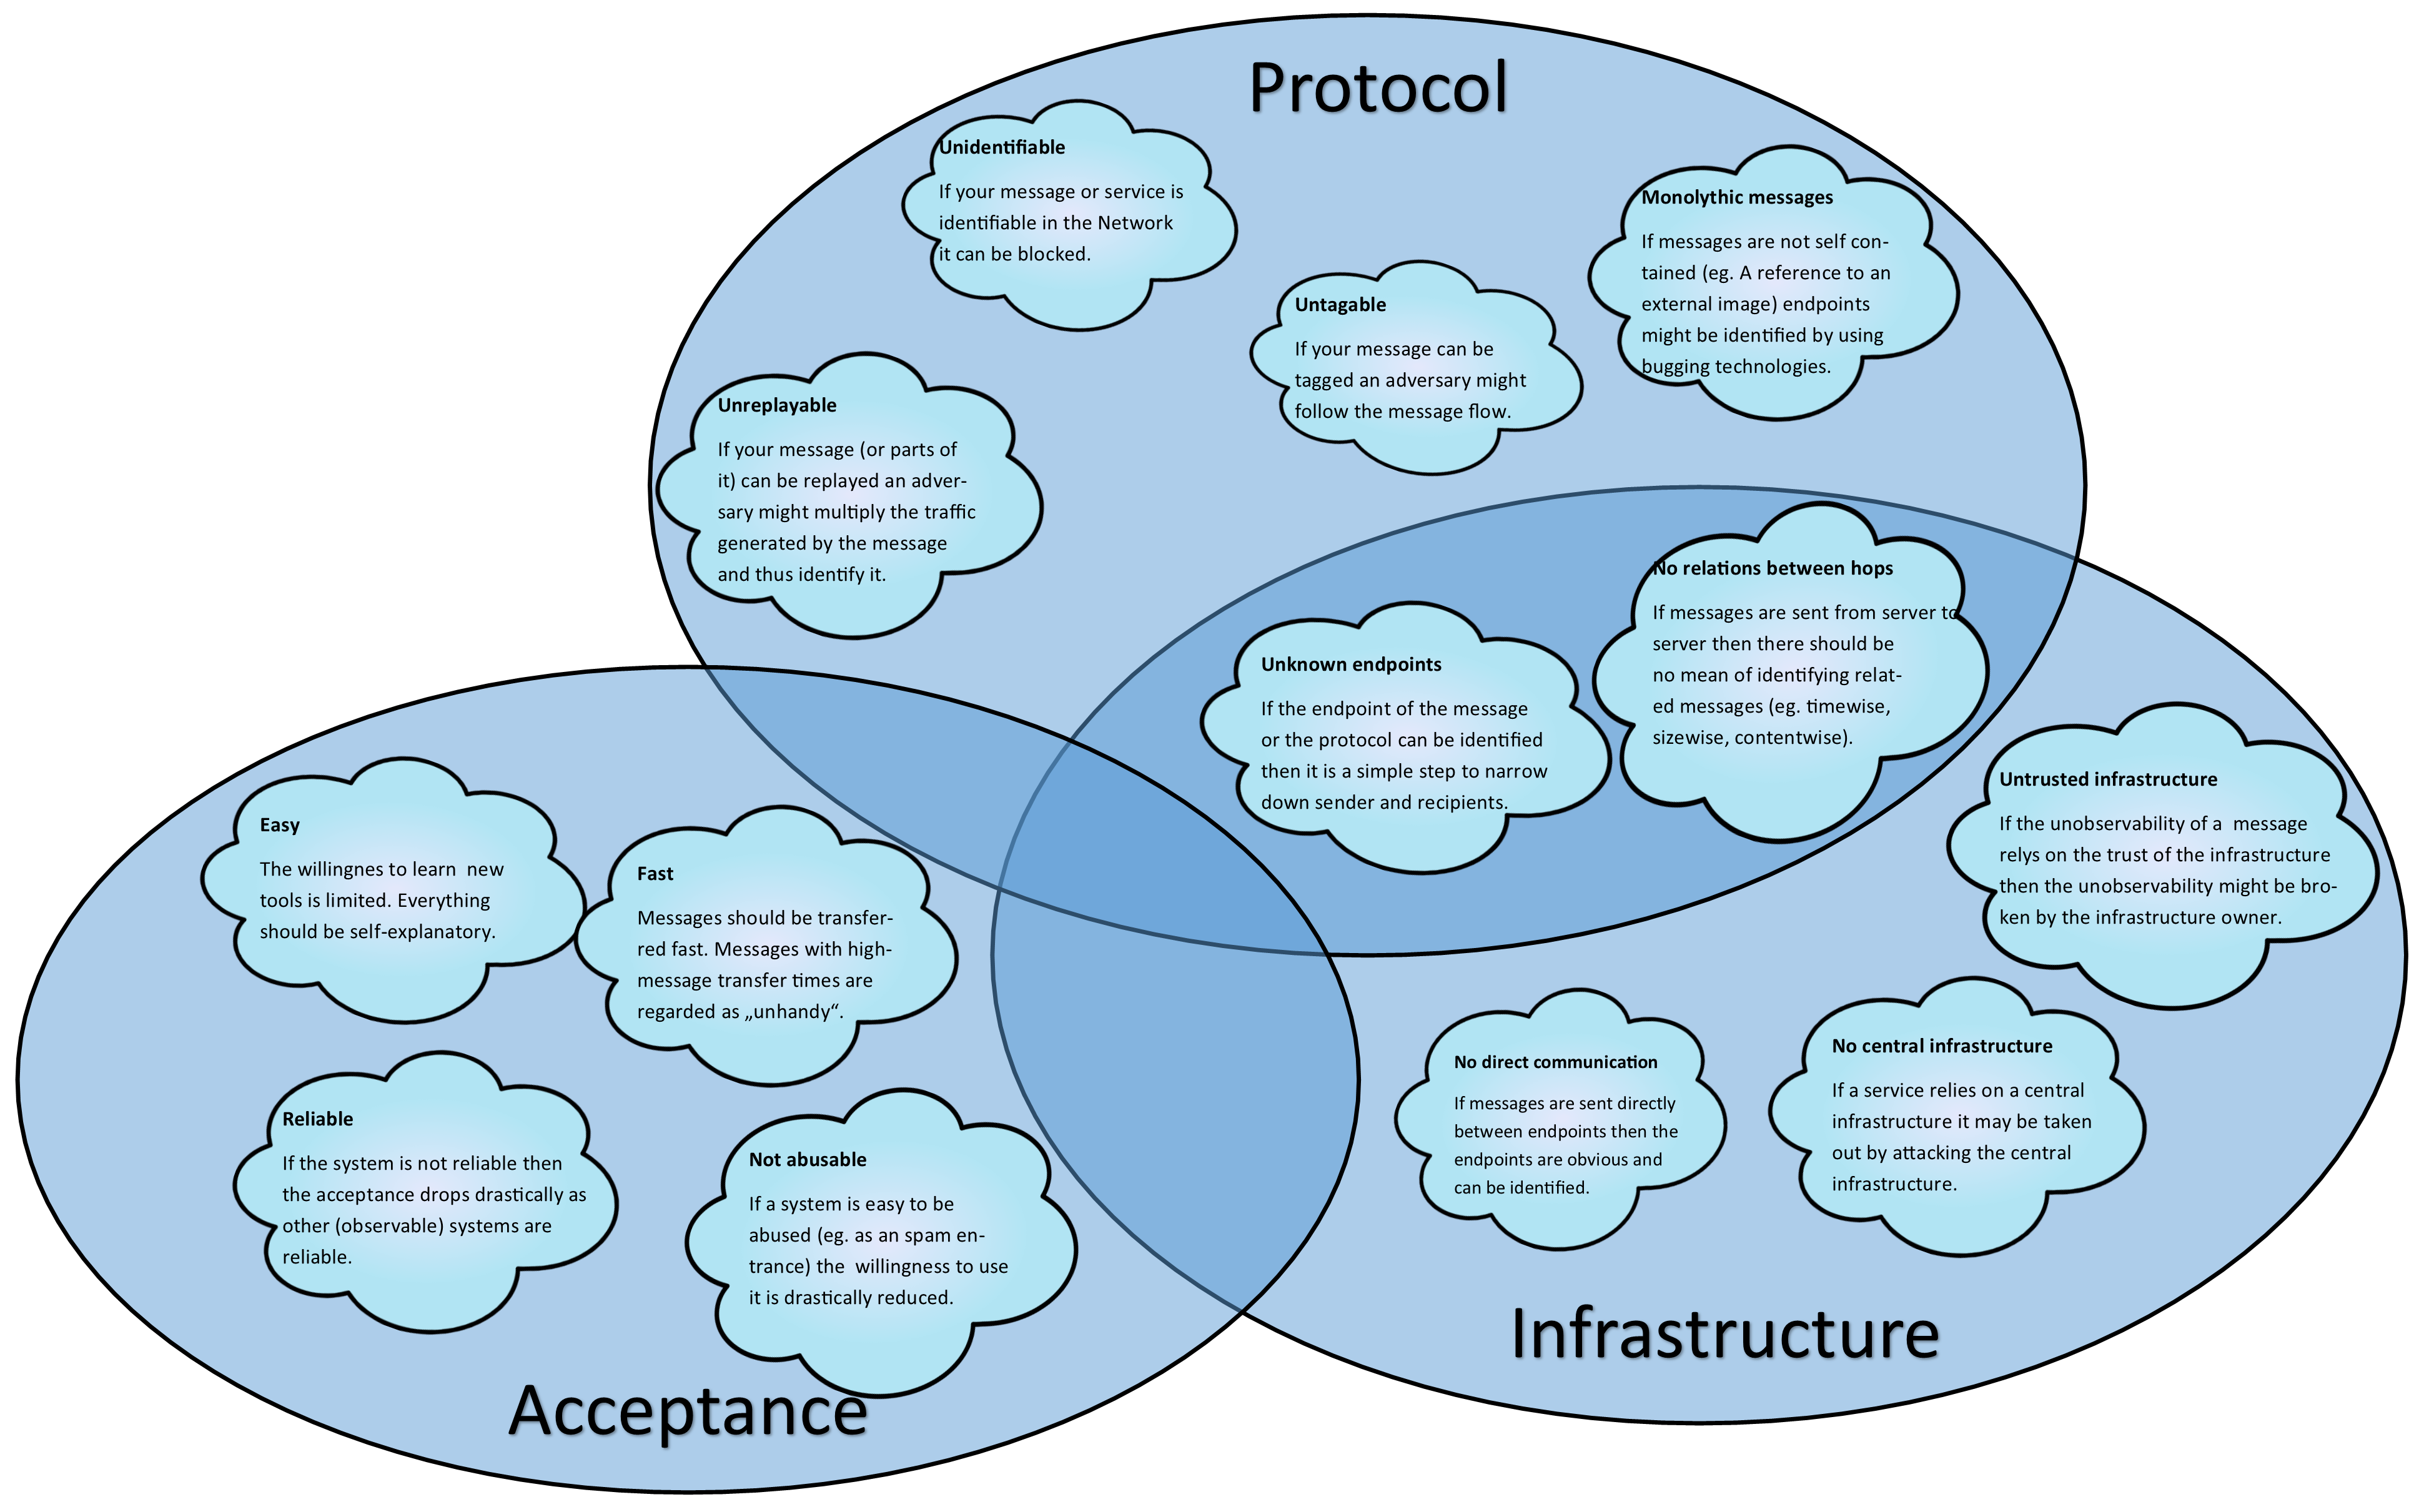
\includegraphics[width=\linewidth]{clouds_full.png}
\caption{Important factors when designing an unobservable message channel}
\end{figure}
\end{alertblock} 
}

%----------------------------------------------------------------------------------------
%	Whats missing
%----------------------------------------------------------------------------------------

\opt{small}{
\begin{block}{What is missing?}
It is still unclear if researchers have done enough research in the past to build an unobservable system. Namely, the research of steganography seems to be in its childhood. Unlike in Cryptology there are no researched “best practices” and no mathematical language for it. We have been unable so far to research the characteristics of covert channels and attributes and we are unable to describe them with scientifically defined attributes in an elaborated language.\\
One thing seems to be clear when looking at the requirements for unobservable system. The costs in terms of bandwidth are tremendous compared to the normal (observable) messages. Cutting the costs of being unobservable should be one of our main goals in future.
\end{block}}
%----------------------------------------------------------------------------------------

\end{column} % End of the second column

\begin{column}{\sepwid}\end{column} % Empty spacer column

\begin{column}{\onecolwid} % The third column

%----------------------------------------------------------------------------------------
%	Infrastructure
%----------------------------------------------------------------------------------------

\begin{block}{Infrastructure}
In order to succeed there are as well certain baselines for the infrastructure:
\begin{itemize}
\item Unknown endpoints\opt{large}{\\
Every endpoint should behave the same as an intermediate routing point. They should receive and send messages so that they are not identifiable as endpoints. Identifiable endpoints simplify analysis.}
\item No relations between single hops\opt{large}{\\
Messages transferred from server to server must be unrelated. Server identifiable to send messages due to received messages are potential targets for analysis.}
\item Untrusted infrastructure\opt{large}{\\
Unlike in a company owned net, in the internet trusting an infrastructure is not possible. It is very often not clear who owns a server and who else does have access to it. So an unobservable system may not build its unobservability based on behavior of the transporting infrastructure.}
\item No central infrastructure\opt{large}{\\
Central infrastructure may be attacked or shut down. They are easier to monitor than an unknown number of participants.}
\item No direct communication between endpoints\opt{large}{\\
If sender and receiver communicate directly then they are easily identified. }
\end{itemize}
\vfill
\end{block}

%----------------------------------------------------------------------------------------
%	ADDITIONAL INFORMATION
%----------------------------------------------------------------------------------------

\begin{block}{Conclusions}
\raggedright
Sending unobservable messages thru a public network is not easy. It cannot be done by inventing a new identifiable service. It has to blend into today's traffic and look unsuspicious compared to all other traffic to be of any value. Yet it has to be easy to handle and simple to understand. Combining today's technologies might be sufficient but have to be researched further.
\vfill
\end{block}

%----------------------------------------------------------------------------------------
%	ADDITIONAL INFORMATION
%----------------------------------------------------------------------------------------

\begin{block}{Additional Information}
\raggedright
For additional information, please see the corresponding papers and presentations published at: {\footnotesize\href{https://www.gwerder.net/\~mgwerder/phd/how\_unobservable/}{https://www.gwerder.net/\textasciitilde mgwerder/phd/how\_unobservable/}} or use the QR code in the top right corner.
\vfill
\end{block}

%----------------------------------------------------------------------------------------
%	REFERENCES
%----------------------------------------------------------------------------------------

\begin{block}{References}

%\nocite{*} % Insert publications even if they are not cited in the poster
\opt{large}{\tiny{\bibliographystyle{unsrt}
\bibliography{../inc/bib/unclassified/Anonbib/anonbib}}}
\opt{small}{\footnotesize{\bibliographystyle{unsrt}
\bibliography{../inc/bib/unclassified/Anonbib/anonbib}}}

\end{block}

\end{column} % End of the third column

\end{columns} % End of all the columns in the poster

\end{frame} % End of the enclosing frame

\end{document}
